\section{Tokenomics}
\label{sec:tokenomics}


{
    \begin{figure*}[htb!]
        \centering
        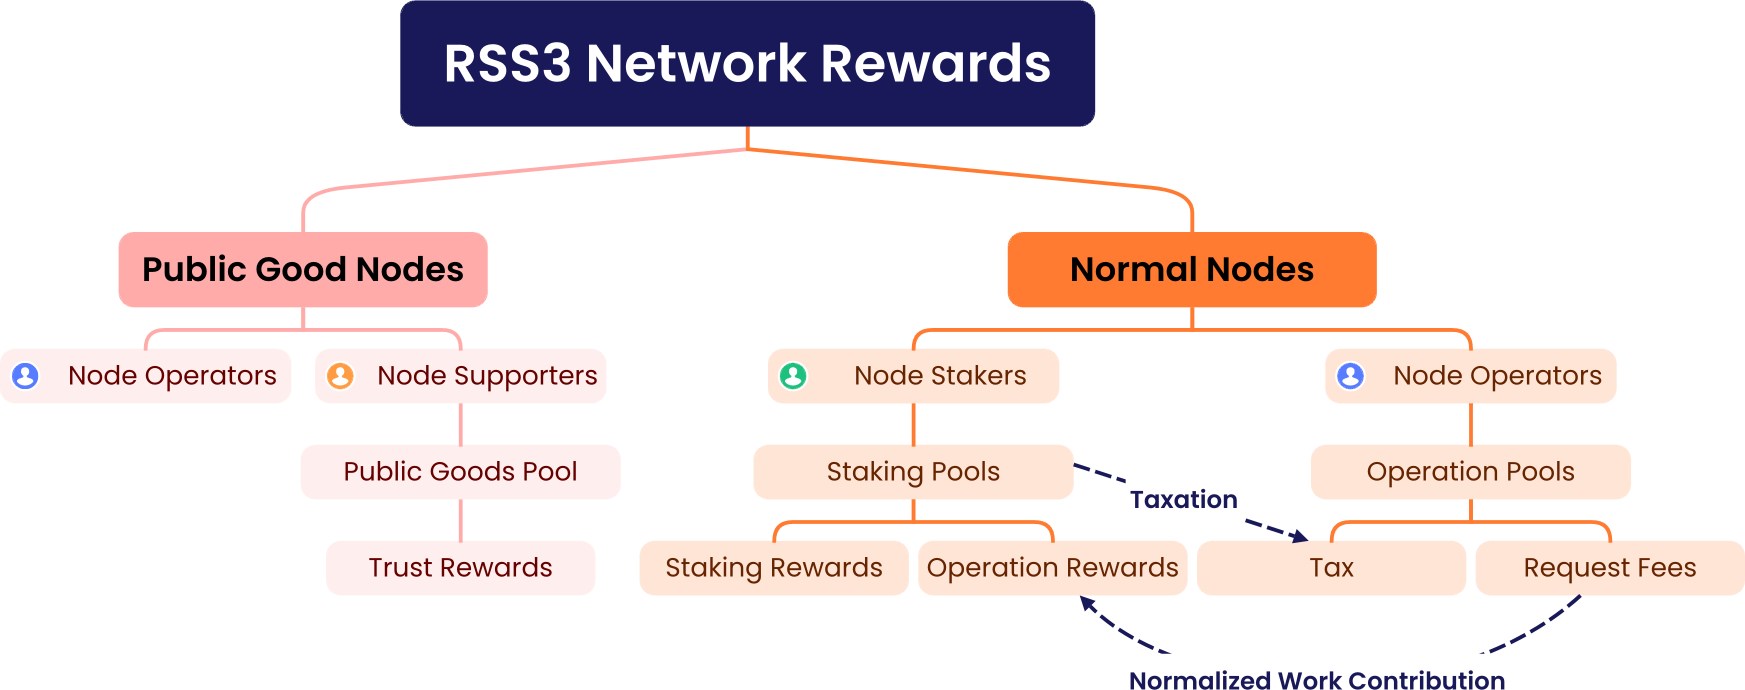
\includegraphics[width=\linewidth]{figures/network-rewards.png}
        \caption{The RSS3 \glsfmtlong{NR} are allocated differently to Normal Nodes and Public Good Nodes.
            See \Cref{subsec:reward_pools} for details.}
        \label{fig:network-rewards}
    \end{figure*}
}


In this seciton, we introduce the detailed tokenomics of the \glsfmtlong{R3N}. We present the concept of Reward Pools, the \glsfmtlong{NR}'s calculation and allocation formulas, and the slashing mechanism employed to enforce the Network's security and stability.

\subsection{Node Operation}
\Glsfmtlong{NO}s are incentivized to operate and maintain the Network by receiving \$RSS3 as rewards.
\begin{enumerate}
    \item Anyone can become a \glsfmtlong{NO} to launch an RSS3 Node and join the RSS3 Network without requiring prior permission.
    \item A \glsfmtlong{NO} has the ability to configure the Node's coverage, which directly influences the Node's capability to respond to various types of requests. A broader coverage means more computational resources are required, and an increased likelihood of receiving requests.
    \item A Node can be operated in either a Normal mode as \node or a Public Good mode as \publicGoodNode. A Normal Node is eligible for \glsfmtlong{NR} but requires a deposit of \$RSS3 into its \operationPool. A Public Good Node is ineligible for \glsfmtlong{NR} but requires no deposit.
    \item A Normal Node has a corresponding \operationPool\ and a \stakingPool. All Public Good Nodes collectively share a single \publicGoodPool.
\end{enumerate}

\subsection{Reward Pools}
\label{subsec:reward_pools}

This section introduces the three reward pools: the \glsfirst{OP}, the \glsfirst{SP}, and the \glsfirst{PGP}. See \Cref{fig:network-rewards} for an illustration.

    {
        \begin{figure*}[htb!]
            \centering
            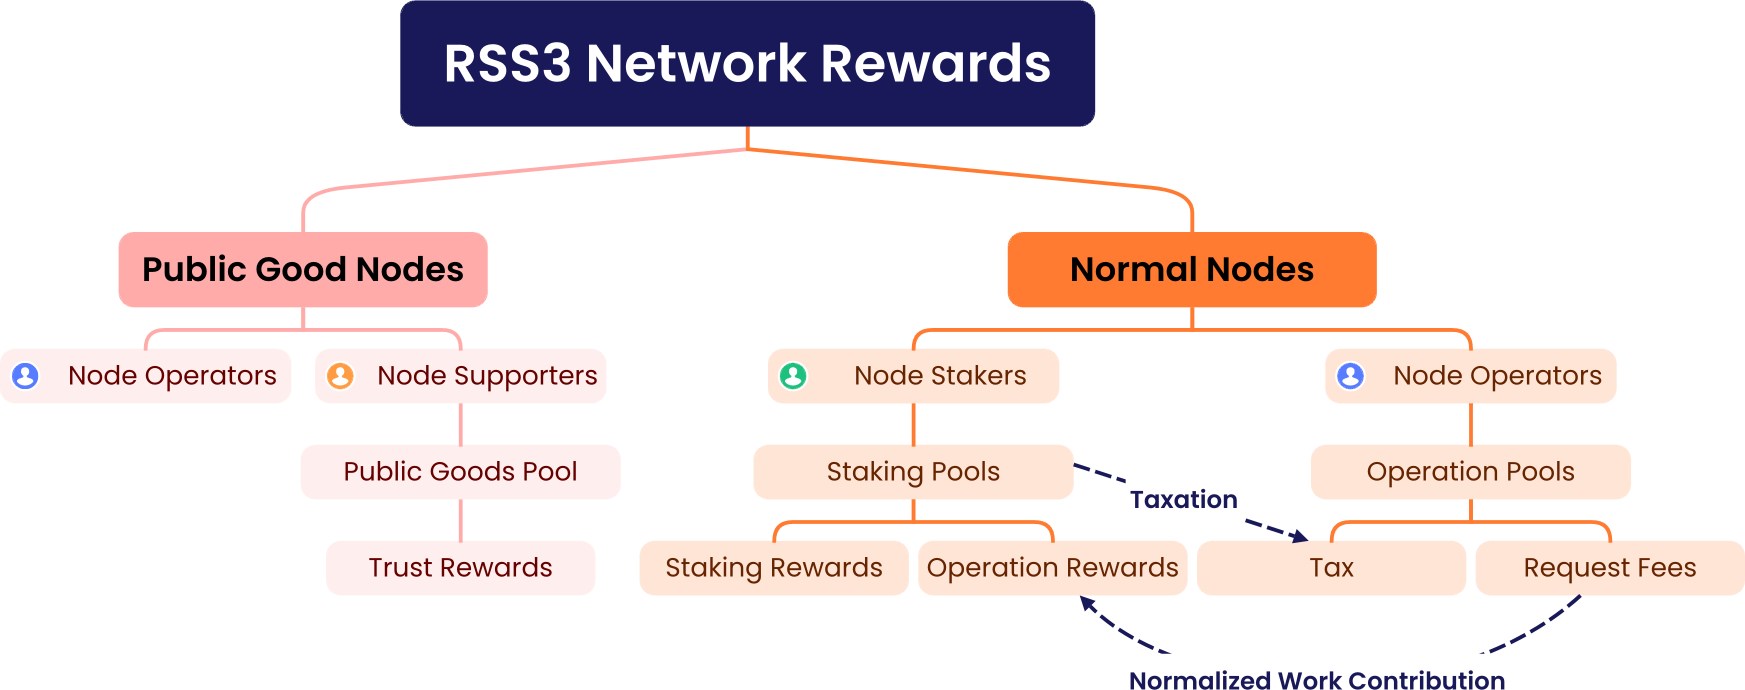
\includegraphics[width=\linewidth]{figures/network-rewards.png}
            \caption{RSS3 \glsfmtlong{NR} allocation.
                The \glsfmtlong{NR} are allocated differently to Normal Nodes and Public Good Nodes.
                See \Cref{subsec:reward_pools} for details.}
            \label{fig:network-rewards}
        \end{figure*}
    }

\subsubsection{\glsfmtlong{OP} (\operationPool)}
\label{subsubsec:operation_pool}

An \glsfirst{OP} is used to store tokens that are allocated to a Normal Node from two sources:
\begin{enumerate}
    \item The \gls{Fee} collected from requests served on the \gls{DSL}
    \item The \gls{Tax} collected from the Node's \stakingPool
\end{enumerate}

The \glsfmtlong{NO} can set a tax rate, \taxRate, which is applied to its \stakingPool.
The tax applies to the \glsfmtlong{NR} allocated to the Node's \stakingPool, not the staked tokens. See \Cref{subsubsec:taxation}.

Only the corresponding \glsfmtlong{NO} can withdraw tokens from its \operationPool, and the withdrawal is subject to a waiting period imposed by the Network.

\subsubsection{\glsfmtlong{SP} (\stakingPool)}
\label{subsubsec:staking_pool}

A \glsfirst{SP} is used to store staked tokens for a Normal Node. Network participants can stake tokens into a Normal Node's \stakingPool\ to increase the Node's chance to receive requests on the \gls{DSL}.

The allocation of \glsfmtlong{NR} into a Node's \stakingPool\ at the end of each epoch \epoch, is determined by two factors:
\begin{enumerate}
    \item \gls{OR}, the Node's normalized work contribution \work\ in proportion to the total work done on the \gls{DSL} (See \Cref{subsubsec:staking_rewards})
    \item \gls{SR}, the Node's \stakingPool\ size in proportion to the total staked tokens on the \gls{VSL} (See \Cref{subsubsec:operation_rewards})
\end{enumerate}

A tax \tax\ is then applied to the received Rewards, with the rate set by its \glsfmtlong{NO}.

\subsubsection{\glsfmtlong{PGP} (\publicGoodPool)}

A \glsfirst{PGP} is a unique reward pool that is shared by all Public Good Nodes.

As Public Good Nodes do not have their own \stakingPool, network participants entrust their tokens to the \publicGoodPool\ and signify their support to a designated Public Good Node.


\subsection{Staking, Trust and Chip}
Network participants are incentivized to secure and improve the Network with their \$RSS3 tokens.

\subsubsection{Staking}

A Normal Node accepts staking into its \stakingPool, the amount of staked \$RSS3 signifies its quality and reliability, this increases the likelihood of receiving requests for a Node.

\subsubsection{Trust}

A Public Good Node does not have a \glsfmtlong{SP} and does not participate in any form of incentivization. Instead, network participants may choose to entrust such a Node, and their tokens are stored into a \glsfmtlong{PGP}. The trust level affects the likelihood of routing requests to a Public Good Node.

\subsubsection{Chip}

A Chip \chip\ is an ERC-721 Non-Fungible Tokens (NFTs) representing a network participant's stake in a particular Node.
When a network participant stakes or entrusts tokens to a Node \node, the participant automatically receives Chips RSS3-\node\ ($\chip_\node$).

\paragraph{Minting}
The number of Chips minted for a particular staking or entrusting \staking\trust\ is determined by:

\begin{equation}
    \label{eq:chip_supply}
    \chip_{\node_\text{mint}} = 
    \frac{\staking\trust * \max(1, \chip_{\node_\text{total}})}{\stakingPool}
\end{equation}

Where $\chip_{\node_\text{mint}} \in \mathbb Z_{> 0}$ is always a non-negative integer.

\paragraph{Redemption}
A Chip can be redeemed for its underlying staked or entrusted tokens at any time, subject to a waiting period imposed by the Network.
The redemption amount may be different from the original staking or entrusting amount due to the change of the underlying \stakingPool\ balance, which follows the same formula as \Cref{eq:chip_supply}:

\begin{equation}
    \label{eq:chip_redeem}
    \staking\trust_{\text{redeem}} = 
    \frac{\chip_{\node_\text{redeem}} * \stakingPool}{\max(1, \chip_{\node_\text{total}})}
\end{equation}

% {
% \renewcommand{\arraystretch}{1.5}
% \begin{table*}[h]
%     \resizebox{\textwidth}{!}{
%         \begin{tabulary}{\textwidth}{|p{6cm}|p{5cm}|p{5cm}|}
%             \hline
%             & \textbf{Node in Normal Mode} & \textbf{Node in Public Good mode} \\ \hline

%             Who can operate? &
%             Anyone &
%             Anyone \\ \hline

%             Is a deposit required for operating a Node? &
%             Yes &
%             No \\ \hline

%             Is the deposit considered as staking, making it eligible for rewards from its own \stakingPool? &
%             No &
%             N/A \\ \hline

%             Will the Node be slashed? &
%             Yes, its deposit and \stakingPool will be slashed. A Node may be demoted to receive fewer requests.
%             & No, but a Node may be demoted to receive fewer requests. \\ \hline

%             Does the Node accept staking? &
%             Yes. The staked tokens go to the Node’s \stakingPool. RSS3-X (X being the Node’s name) Chips are issued to the stakers after staking. &
%             No, as such a Node does not have a \stakingPool. Instead, stakers stake to the \publicGoodPool. RSS3-Public Good Chips are issued to the stakers after staking. \\ \hline

%             Can the \glsfmtlong{NO} set a tax \taxRate? &
%             Yes &
%             No, a universal tax is determined by the Network. \\ \hline

%             Does it have an \glsfmtlong{OP} \operationPool? &
%             Yes &
%             No, its \glsfmtlong{OR} go to [X] \\ \hline

%             Does it have a \glsfmtlong{SP} \stakingPool? &
%             Yes &
%             No, but a \glsfmtlong{PGP} with a universal incentive rate. \\ \hline
%         \end{tabulary}
%     }
%     \caption{Comparison of two Node Operation modes.}
%     \label{table:node_modes}
% \end{table*}
% }

\subsection{\glsfmtfull{NR}}
\label{subsec:network_rewards}

In \Cref{sec:VSL}, we describe the intentions behind the \gls{VSL}'s incentive mechanism, here we introduce the detailed \glsfmtlong{NR} calculation and distribution formulas separately.

The \glsfmtlong{NR} \networkReward\ consists of three parts:
\begin{equation}
    \label{eq:network_rewards}
    \networkReward = (\operationReward + \stakingReward) + \trustReward
\end{equation}

See \Cref{fig:network-rewards} for an illustration. The allocation to each part is determined by the Network, and is subject to potential future changes.

\subsubsection{\glsfmtfull{OR}}
\label{subsubsec:operation_rewards}

To encourage Normal Nodes to operate reliably and consistently to maintain the Network, \operationReward\ is allocated to a Node's \operationPool\ in proportion to its \glsfirst{Fee} collected on the \gls{DSL} during the last \epoch.

\begin{equation}
    \label{eq:operation_weight}
    \work_\nodeAtEpoch =
    \log_{2}
    (
    \frac{\fee_\nodeAtEpoch}
    {\sum_{x=0}^{\infty} \fee_{x, \epoch}} + 1
    ) * G
\end{equation}

$\work_\nodeAtEpoch$ denotes the normalized work contribution for a given Normal Node \node, at the end of a given epoch $\epoch$. $G$ is a constant equal to $\ln(2) \approx 0.693147$ used to offset the effect of replacing $\ln$ with $\log_2$, as the former is more costly in terms of gas when it comes to on-chain computation.

\begin{equation}
    \label{eq:operation_rewards}
    \networkReward_{\operation|\node, \epoch} =
    \frac{\work_\nodeAtEpoch}
    {\sum_{x=0}^{\infty} \work_{x, \epoch}}
    * \networkReward_{\operation, \epoch}
\end{equation}

$\networkReward_{\operation|\node, \epoch}$ therefore denotes the Operation Rewards for a given Normal Node \node, at the end of a given epoch $\epoch$.

\subsubsection{\glsfmtfull{SR}}
\label{subsubsec:staking_rewards}

To encourage participation from all network participants to increase the Network's reliability, \stakingReward\ is allocated to a Normal Node's \stakingPool\ in proportion to the amount of staked tokens in the entire Network during the last \epoch.

\begin{equation}
    \label{eq:staking_rewards}
    \networkReward_{\staking|\node, \epoch} =
    \frac{\pool_{\staking|\node, \epoch}}
    {\sum_{x=0}^{\infty} \pool_{\staking|x, \epoch}}
    * \networkReward_{\staking, \epoch}
\end{equation}

$\networkReward_{\staking|\node, \epoch}$ therefore denotes the Staking Rewards for a given Normal Node \node, at the end of a given epoch $\epoch$.

\subsubsection{\glsfmtfull{TR}}

To encourage participation from all network participants to increase the Network's reliability and support Public Goods provision, \trustReward\ is allocated to the \publicGoodPool\ in proportion to the amount of entrusted tokens in the entire Network during the last \epoch.

\begin{equation}
    \label{eq:trust_rewards}
    \networkReward_{\trust|\node, \epoch} =
    \frac{\pool_{\trust|\node, \epoch}}
    {\sum_{x=0}^{\infty} \pool_{\trust|x, \epoch}}
    * \networkReward_{\trust, \epoch}
\end{equation}

$\networkReward_{\trust|\node, \epoch}$ therefore denotes the \glsfmtlong{TR} for a given Public Good Node \node, at the end of a given epoch $\epoch$.

\subsubsection{Taxation (\tax)}
\label{subsubsec:taxation}

The tax rate \taxRate\ is set by the \glsfmtlong{NO} of a Normal Node, and is applied to the \glsfmtlong{NR} allocated to its \stakingPool.
The amount of tax collectible is capped at a maximum of \taxCap\ times the amount of the current deposit. \taxCap\ is set by the Network.

\begin{equation}
    \tax_{\node, \epoch} =
    \min(\deposit_{\node, \epoch}
    * \taxCap_\epoch , (\networkReward_{\staking|\node, \epoch}
    + \networkReward_{\operation|\node, \epoch} ) 
    * \taxRate_{\node, \epoch})
\end{equation}

\subsubsection{Final Allocations}
\label{subsubsec:allocation}

The total amount of tokens allocated to a Normal Node's \operationPool\ for a given epoch $\epoch$ is therefore:

\begin{equation}
    \fee_{\node, \epoch}
    + \tax_{\node, \epoch}
\end{equation}

The total amount of tokens allocated to a Normal Node's \stakingPool\ for a given epoch $\epoch$ is therefore:

\begin{equation}
    \networkReward_{\operation|\node, \epoch}
    + \networkReward_{\staking|\node, \epoch}
    - \tax_{\node, \epoch}
\end{equation}

The total amount of tokens allocated to a Public Good Node's \publicGoodPool\ for a given epoch $\epoch$ is therefore:

\begin{equation}
    \networkReward_{\trust|\node, \epoch}
\end{equation}

\subsection{Slashing}

Slashing is a mechanism used to enforce the Network's security and stability. It is applied to both Normal Nodes and Public Good Nodes, albeit in slightly different ways.

A slashing occurs when a Node fails to meet the requirements set by the Network. This can be due to a variety of reasons, including but not limited to: 1) the Node is offline for an extended period of time; 2) the Node is not serving requests in a timely manner; 3) the Node is serving requests but with incorrect information.

Should a slashing occur, the Node's \deposit\%, \stakingPool\%, and \networkReward\ will be slashed by precentages determined by the Network.
The Node's \reliabilityScore\ will be negatively impacted, diminishing its likelihood of receiving requests on the \gls{DSL}.

The disposition of the slashed tokens is as follows:
\begin{itemize}
    \item a portion of the slashed tokens will be burned, the amount is determined by the Network
    \item a portion of the slashed tokens will go to the reporter, provided the Node’s misconduct was not auto-detected by the Network
    \item the remaining portion of the slashed tokens will go to the \publicGoodPool
\end{itemize}

% TODO: add slashing into formulas7
